% app1.tex (will be Appendix A)

%\label{app:proof}

%\newpage
%\section{Proof of Lemma~\ref{easylemma}}
%\label{app:proof:easy}

%\noindent \textbf{Proof}:\quad The result is clearly obvious.

%\setcounter{secnumdepth}{1}
%\setcounter{section}{0}
\chapter{Simple Examples of Collective Modes Frequencies in Presence of Interactions}
\section{Non-Local Interaction, $|n\rangle,|n+1\rangle$ Pair}
\label{Notes on unpublished calculations}
\setcounter{equation}{0}

\subsection{Calculation of Self-Energy}
We know,
\begin{equation}
G^{-1} = G_0^{-1} - \Sigma
\end{equation}
\begin{equation}
G = \frac{1}{{G_0^{-1}-\Sigma}}=\frac{G_0}{{1-G_0\Sigma}}=G_0(1+G_0\Sigma+G_0\Sigma G_0\Sigma)
\end{equation}
\begin{equation}
G=G_0 + G_0\Sigma G_0 + G_0\Sigma G_0\Sigma G_0
\end{equation}
We need to compute \(\Sigma\) to the leading order according to Fock approximation. \newline
The quantity, \[\delta
\langle\Psi\Psi^\dagger\rangle=\langle \Psi| -\int_0^\beta{d\tau\mathcal{H}_I}|\Psi^\dagger \rangle \]
\[\mathcal{H}_I=V\Psi^\dagger \Psi^\dagger \Psi \Psi \]
\[\delta\langle\Psi \Psi^\dagger \rangle = \langle \Psi| (-V) \Psi^\dagger \Psi^\dagger \Psi \Psi |\Psi^\dagger \rangle = -V \langle \Psi | \Psi^\dagger \Psi^\dagger \Psi \Psi | \Psi^\dagger \rangle = -V \langle \Psi \Psi^\dagger \rangle \langle \Psi \Psi^\dagger \rangle \langle \Psi \Psi^\dagger \rangle\]
\[\delta G = \delta \langle - \Psi \Psi^\dagger \rangle = (-)-V \langle -\Psi \Psi^\dagger \rangle \langle -\Psi \Psi^\dagger \rangle \langle -\Psi \Psi^\dagger \rangle (-1)^3 = V G_0 G_0 G_0 = \delta G\]

\begin{equation}
\Rightarrow \Sigma = -VG_0
\end{equation}
Thus, the sign is fixed. \newline \newline
In case of 2D gas,
\begin{equation}
\Sigma_{p,i\omega_n}=-\int{T\sum\limits_{\epsilon_n} V_q G_0(p+q,\epsilon_n+\omega_n)}
\end{equation}
In the (y,k) representation
\begin{equation}
G(y_1,y_2;k)=\sum\limits_m \frac{\Psi_m(y_1)\Psi_m^*(y_2)}{i\epsilon_n-E_{mk}}=\sum\limits_m \Psi_m(y_1)\Psi_m^*(y_2)G_m(\epsilon_n,k)
\end{equation}

\[E_{mk}=\omega_{\perp}(m+\frac{1}{2})+\frac{k^2}{2}; \; \; \; \xi_{mk}=E_{mk}-\mu\]

\begin{equation}
\begin{split}
\sum\limits_m(p,i\omega_n)=-\int{\frac{dq}{2\pi}T\sum\limits_{\epsilon_n}\sum\limits_{m'}}
& {\int{dy_1}\int{dy_2}} \\
& {V_q(y_1-y_2)\Psi_m(y_1)\Psi_{m'}(y_1)\Psi{m'}(y_2)\Psi_m(y2)\,G_m(\epsilon_n,k+q)e^{i\epsilon_n0^+}}
\end{split}
\end{equation}

\[T\sum\limits_{\epsilon_n}f(i\epsilon_n)=\oint_\Gamma\frac{dz}{2\pi i}f(z)n_F(z)\]

\[\frac{1}{e^{\beta z}+1};\ \ z=\frac{2\pi}{\beta}(n+\frac{1}{2})i+\delta z=z_n+\delta z\]

\[e^{\beta z}+1=e^{2\pi (n+\frac{1}{2})i+\delta z \beta}=(-1)e^{\beta\delta z}+1=-(1+\beta \delta z)+1=-\beta \delta z \]

\[\Rightarrow \frac{1}{e^{\beta z}+1}\approx \frac{1}{-\beta\delta z}=-\frac{1}{\beta}\frac{1}{\delta z}=-T\frac{1}{\delta z}\]

thus, \[T\sum\limits_{\epsilon_n}\frac{e^{i\epsilon_n0^+}}{i\epsilon_n-\xi}=-\oint_\Gamma\frac{dz}{2\pi i}n_F(z)\frac{e^{z0+}}{z-\xi}=\oint_{z=\xi}\frac{dz}{2\pi i}n_F(z)\frac{1}{z-\xi}=n_F(\xi)\]

or,
\begin{equation}
T\sum\limits_{\epsilon_n}\frac{e^{i\epsilon_n0^+}}{i\epsilon_n-\xi}=n_F(\xi)
\end{equation}

thus, \be \Sigma_m(p,i\omega_n)=-\int{\frac{dq}{2\pi} \sum\limits_{m'}\int{dy_1}\int{dy_2}V_q(y_1-y_2)\Psi_m(y_1)\Psi_{m'}(y_1)\Psi_{m'}(y_2)\Psi_m(y_2)n_F(\xi_{m',k+q})} \ee
we approximate the potential of the form
\be V_q(y_1-y_2)=V_0[cos(q_\perp(y_1-y_2))-1]\approx \frac{1}{2}V_0q_\perp^2(y_1-y_2)^2 \ee
as there is no dependence of V on momentum transferred along the guide, we can just integrate over
\[\int{\frac{dq}{2\pi}n_F(\xi_{m,k+q})}=\frac{2k_F^m}{2\pi}=\frac{k_F^m}{\pi}\]
which is the total number of electrons in the subband m.\\
Finally,
\be \Sigma_m(p,i\omega_n)=-\frac{1}{2}V_0q_\perp^2\sum\limits_{m'}\int{dy_1}\int{dy_2}(y_1-y_2)^2\frac{k_F^{m'}}{\pi}\Psi(y_1)\Psi_{m'}(y_1)\Psi_{m'}(y_2)\Psi(y_2) \ee

\subsection{Calculation of Polarization Operator}
let's first compute the following quantity:
\[T\sum\limits_m G_m(i\epsilon_n+i\omega_n,p+q)G(i\epsilon_n,p)\]
\[=\,T\sum\limits_n \frac{1}{i\epsilon_n+i\omega_n-\xi_1}\frac{1}{i\epsilon_n-\xi_2}\]
\[=\,-\oint_\Gamma \frac{dz}{2\pi i}n_F(z)\frac{1}{z+i\omega_n-\xi_1}\frac{1}{z-\xi_2}\]
\[=\,\frac{n_F(\xi_1-i\omega_n)}{\xi_1-\xi_2-i\omega_n}+\frac{n_F(\xi_2)}{\xi_2-\xi_1+i\omega_n}\]
\[=\,\frac{n_F(\xi_2)-n_F(\xi_1)}{\xi_2-\xi_1+i\omega_n}\]
now,
\[\Pi_{n-1}{n}=\,T\sum\limits_{\epsilon_n}\int{\frac{dp}{2\pi}G^n(i\epsilon_n+i\omega_n,p)G^{n-1}(i\epsilon_n,p)}\]
\[=\,\int{\frac{dp}{2\pi}\frac{n_F(\xi_p^{(n-1)})-n_F(\xi_p^n)}{\xi_p^{(n-1)}-\xi_p^n+i\omega_n}}\]
\[\xi_p^n=\;\frac{k^2}{2}+\omega_{\perp}(n+\frac{1}{2})+\Sigma_n\]

thus,
\be \Pi_{n-1}^n=\;\frac{1}{\pi}\frac{k_F^{n-1}-k_F^n}{-\omega_{\perp}-(\Sigma_n-\Sigma_{n-1})+i\omega_n} \ee

% \bd \includegraphics[scale=1]{slv11.jpg} \ed

\subsection{One Level Occupied}

\be \Sigma_0=- \piinv \C k_F^0 \ee

\be \Sigma_1= \piinv \C k_F^0 \ee

If we let $\omega \rightarrow \omega_{\perp}$,
\be \Pi_0^1 = \frac{1}{\pi} \frac{k_F^0}{\Sigma_0-\Sigma_1} = - \frac{\omega_{\perp}}{V_0q_\perp^2} \ee
Interaction, 
\be V=-\frac{1}{2}V_0q_\perp^2 ( \langle 1|y^2|1\rangle + \langle 0|y^2|0 \rangle) =-\frac{V_0q_\perp^2}{\omega_{\perp}} \ee
Thus, \be V\Pi = 1 \\ \ee


\subsection{Two Levels Occupied}
\be \Sigma_0= -\piinv \C (k_F^0-k_F^1) \ee
\be \Sigma_1 = -\piinv \C (-k_F^0+3k_F^1) \ee
\be \Sigma_2 = -\piinv \C (-2k_F^1) \ee
\be \Pi_1=\piinv \frac{k_F^0-k_F^1}{\Sigma_0-\Sigma_1}=\frac{k_F^0-k_F^1}{-\C (2k_F^0-4k_F^1)}\ee
\be\Pi_2=\piinv \frac{k_F^1-k_F^2}{\Sigma_1-\Sigma_2}=\frac{k_F^1}{-\C (-k_F^0+5k_F^1)} \ee
Thus, \be \Pi=-\frac{1}{\C} 
\left ( \begin{array}{cc}
\frac{k_F^0-k_F^1}{-\C (2k_F^0-4k_F^1)} & 0 \\
0 & \frac{k_F^1}{-\C (-k_F^0+5k_F^1)} \\
\end{array}
\right) \ee

\be V_{11}=-\frac{1}{2}V_0q_\perp^2(\langle 0|y^2|0 \rangle + \langle 1|y^2|1 \rangle ) = -\C.2\ee
\be V_{12}=-\frac{1}{2}V_0q_\perp^2(-1\langle 0|y|1\rangle \langle 1|y|2 \rangle)=\C.\sqrt{2}\ee
\be V_{22}=-\frac{1}{2}V_0q_\perp^2(\langle 1|y^2|1 \rangle + \langle 2|y^2|2 \rangle ) = -\C.4 \ee
\be V=-\C \left (\begin{array}{cc} 2 & -\sqrt{2} \\ -\sqrt{2} & 4 \\ \end{array} \right) \ee
Simple calculation yields: \be det[\mathbbm{1}-V\Pi]=0 \\ \ee

\subsection{Three Levels Occupied}
\be \Sigma_0= -\piinv \C (k_F^0 -k_F^1) \, (Same\ as\ before)\ \ee
\be \Sigma_1\ has\ an\ additional\ part:\ =\piinv\C.2k_F^2 \ee
\be \Rightarrow\Sigma_1=-\piinv\C(-k_F^0+3k_F^1-2k_F^2) \ee
\be \Sigma_2\ has\ an\ additional\ part:\ =-\piinv\C(-2k_F^1+5k_F^2) \ee
\be \Sigma_3=-\piinv\C(-3k_F^2) \ee

\be \Pi_0=\piinv\frac{k_F^0-k_F^1}{\Sigma_0-\Sigma_1}=\frac{k_F^0-k_F^1}{-\C(2k_f^0-4k_F^1+2k_F^2)} \ee
\be \Pi_1=\piinv\frac{k_F^1-k_F^2}{\Sigma_1-\Sigma_2}=\frac{k_F^1-k_F^2}{-\C(-k_F^0+5k_F^1-7k_F^2)} \ee
\be \Pi_2=\piinv\frac{k_F^2-k_F^3}{\Sigma_2-\Sigma_3}=\frac{k_F^2}{-\C(-2k_F^1+8k_F^2)} \ee
Thus, \be \\ \Pi=\left(\begin{array}{ccc}
									\frac{k_F^0-k_F^1}{-\C(2k_f^0-4k_F^1+2k_F^2)} & 0 & 0\\
									0 & \frac{k_F^1-k_F^2}{-\C(-k_F^0+5k_F^1-7k_F^2)} & 0\\
									0 & 0 & \frac{k_F^2}{-\C(-2k_F^1+8k_F^2)} \end{array} \right ) \ee
\be V_{11}=-\C.2\ (as\ before) \ee
\be V_{12}=\C.\sqrt{2}=V_{21}\ (as\ before)\ \ee
\be V_{13}=0=V_{31}\ee
\be V_{22}=-\C.4\ (as\ before) \ee
\be V_{23}=-\frac{1}{2}V_0q_\perp^2(-2\langle 2|y|3 \rangle \langle 1|y|2 \rangle)=\C.\sqrt{6}=V_{32} \ee
\be V_{33}=-\frac{1}{2}V_0q_\perp^2(\langle 3|y^2|3 \rangle + \langle 2|y^2|2 \rangle)=-\C.6 \ee
\be V=-\C \left (\begin{array}{ccc}
							2 & -\sqrt{2} & 0 \\
							-\sqrt{2} & 4 & -\sqrt{6} \\
							0 & -\sqrt{6} & 6 \end{array} \right ) \ee
After simple calculation, \be \det[\mathbbm{1}-V\Pi]=0 \ee




\section{Non-Local Interaction, $|n,\uparrow\rangle, |n,\downarrow\rangle$ Pair}

\begin{equation}
	H=\frac{p_x^2+p_z^2}{2m_e}+V_c(z)-\frac{1}{2}E_z\sigma_z
\end{equation}
\newline
where,
\begin{equation}
	E_{m,s,k}=\frac{k^2}{2m_e}+(m+\frac{1}{2})\omega_{\perp}-\frac{1}{2}E_zs
\end{equation}

\begin{equation}
G_{m,s}(p,i\omega_n)=\frac{1}{i\omega_n+i\epsilon_n-\xi_{m,s}(p)-\Sigma_{m,s}}
\end{equation}
\newline
Self energies:
\begin{equation}
	\Sigma_{m,s}(p,i\omega_n)=-\int\frac{dq}{2\pi}T\Sigma_{\epsilon_n}\Sigma_{m'}V_q(y_1-y_2)\phi_m(y_1)\phi_{m'}(y_1)\phi_{m'}(y_2)\phi_m(y_2)\frac{e^{i\epsilon_n0^+}}{i\epsilon_n-\xi_{m,s}(p)}
\end{equation}

\[T\sum\limits_{\epsilon_n}\frac{e^{i\epsilon_n0^+}}{i\epsilon_n-\xi_{m,s}(p)}=n_F(\xi_{m,s}(p))\]

\[V(y_a-y_2)=V_0(cos(q_\perp(y_a-y_2))-1\approx\frac{1}{2}V_0q_\perp^2(y_1-y_2)^2\]

\begin{equation}
	\Sigma{m,s}=-\frac{1}{2\pi}V_0 q_\perp^2\sum\limits_{m'}\int{dy_1dy_2}{(y_1-y_2)^2k_F^{m',s}\phi_m(y_1)\phi_m'(y_1)\phi_{m'}(y_2)\phi_m(y_2)}
\end{equation}


Polarization Operator:
\begin{figure}[h]
\begin{center}
	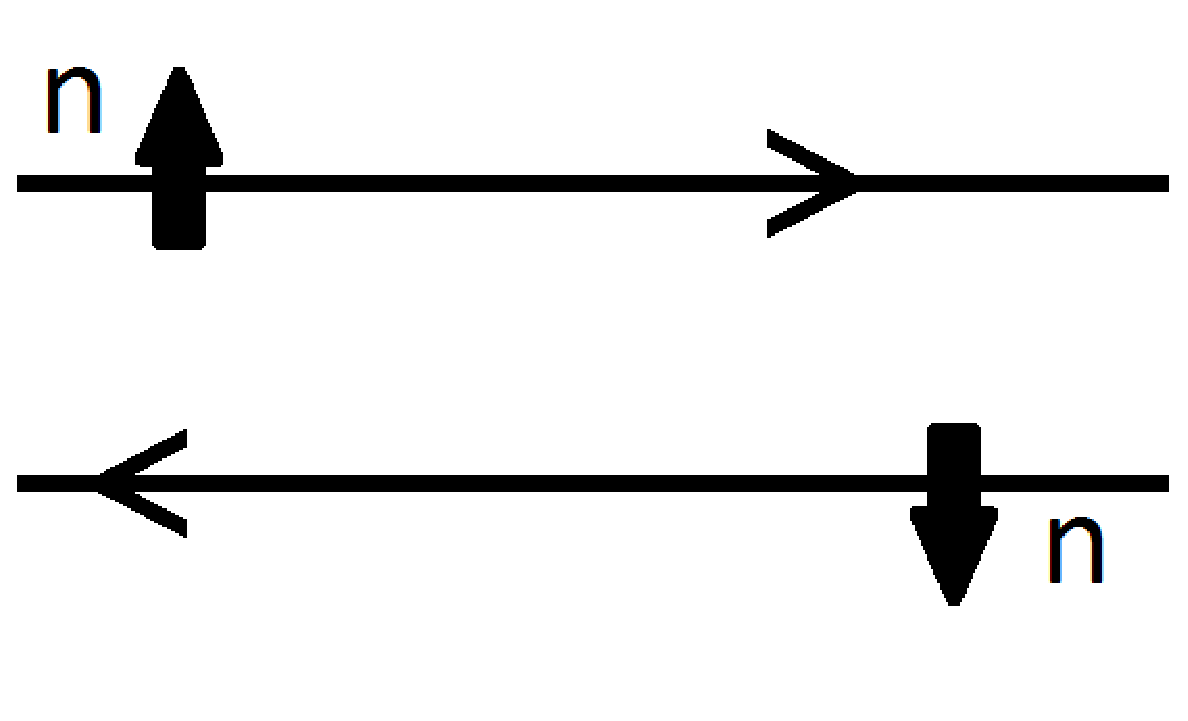
\includegraphics[width=1in]{apfig1}
\end{center}
\end{figure}
\[T\sum\limits_{\epsilon_n}G_{m,s}(i\epsilon_n+i\omega_n,p)G_{m',s'}(i\epsilon_n,p)\]

\[= T\sum\limits_{\epsilon_n} \frac{1}{i\epsilon_n+i\omega_n-\xi_{m,s}(p)-\Sigma_{m,s}} \frac{1}{i\epsilon_n-\xi{m',s'}(p)-\Sigma_{m',s'}}\]

\[=-\oint_\Gamma \frac{dz}{2\pi i} n_F(z) \frac{1}{z+i\omega_n-\xi_{m,s}(p)-\Sigma_{m,s}} \frac{1}{z-\xi_{m',s'}(p)-\Sigma_{m',s'}}\]

\[=\frac{n_F(\xi_{m',s'})-n_F(\xi_{m,s})}{\xi_{m',s'}-\xi_{m,s}+\Sigma_{m',s'}-\Sigma_{m,s}}\]

\[\Pi_{n,\downarrow}^{n,\uparrow}=T\sum\limits_{\epsilon_n} \int \frac{dp}{2\pi} G_{n,\uparrow}(i\epsilon_n+i\omega_n,p)G_{n,\downarrow}(i\epsilon_n,p)\]
or,
\begin{equation}
	\Pi_n=\frac{1}{\pi} \frac{k_F^{n,\downarrow}-k_F^{n,\uparrow}}{i\omega_n-E_z+\Sigma_{n,\downarrow}-\Sigma_{n,\uparrow}}
\end{equation}

Vertex correction:

\[\]

\begin{figure}[h]
	\centering
	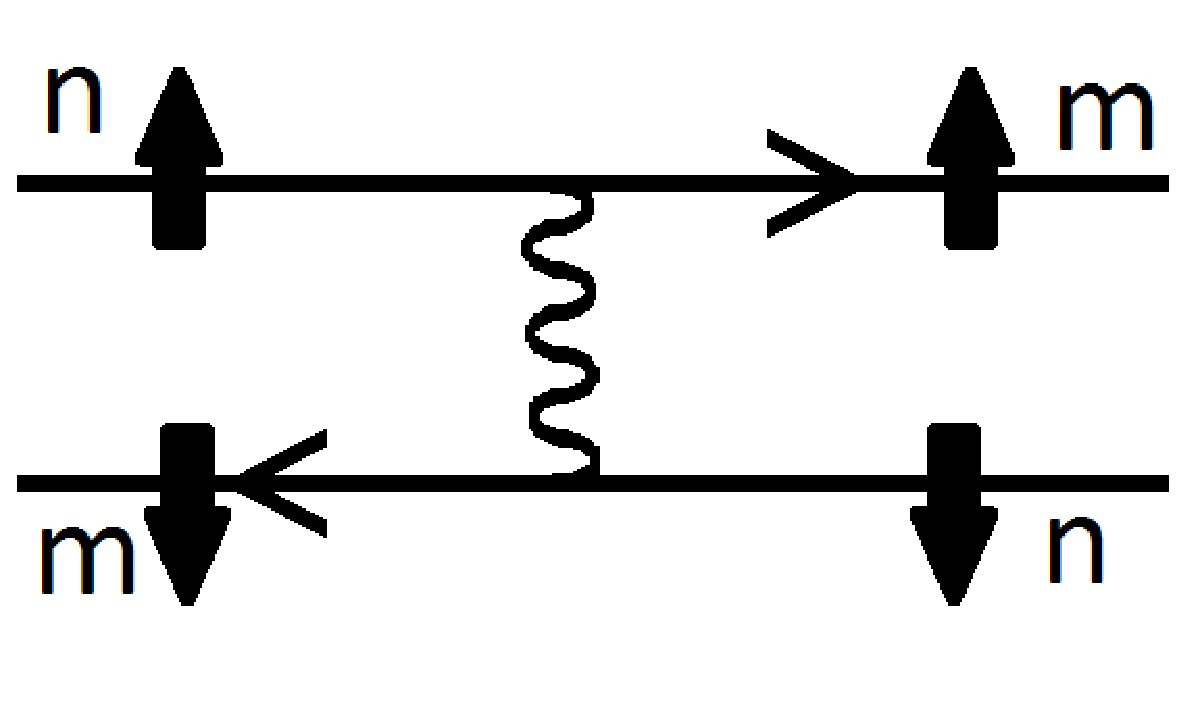
\includegraphics[width=1in]{apfig2}
\end{figure}

\begin{equation}
	V=\frac{1}{2} V_0 q_\perp^2 \int \phi_n(y_1) \phi_m(y_1) (y_1-y_2)^2 \phi_m(y_2) \phi_n(y_2) dy_1 dy_2
\end{equation}

\subsection{One Level Occupied}

\[\Sigma_{0,\uparrow}=-\frac{1}{2\pi} V_0 q_\perp^2 k_F^{0,\uparrow}.2\langle 0|y^2|0\rangle=-\frac{1}{2\pi} \frac{V_0 q_\perp^2}{\omega_{\perp}} k_F^{0,\uparrow}\]

\[\Sigma_{0,\downarrow}=-\frac{1}{2\pi} V_0 q_\perp^2 k_F^{0,\downarrow}.2\langle0|y^2|0\rangle = -\frac{1}{2\pi} \frac{V_0 q_\perp^2}{\omega_{\perp}} k_F^{0,\downarrow}\]


\[\Pi|_{\omega\rightarrow E_z}=\frac{\frac{1}{\pi}(k_F^{0,\downarrow}-k_F^{0,\uparrow})}{\Sigma_{0,\downarrow}-\Sigma_{0,\uparrow}}=\frac{\frac{1}{\pi}(k_F^{0,\downarrow}-k_F^{0,\uparrow})}{-\frac{1}{2\pi} \frac{V_0 q_\perp^2}{\omega_{\perp}}(k_F^{0,\downarrow}-k_F^{0,\uparrow})}=-\frac{2\omega_{\perp}}{V_0 q_\perp^2}\]

\[V=\frac{1}{2} V_0 q_\perp^2. 2\langle 0|y^2|0\rangle = \frac{V_0 q\perp^2}{2\omega_{\perp}} \]

\[\mathbb{I}+V\Pi=1-1=0\]

\subsection{Two Levels Occupied}

\[\Sigma_{0,\uparrow}=-\frac{1}{2\pi} V_0 q_\perp^2 \{k_F^{0,\uparrow}.2\langle 0|y^2|0\rangle + k_F^{1,\uparrow}.(-2)|\langle 0|y|1\rangle|^2\}=-\frac{1}{2\pi} \frac{V_0 q_\perp^2}{\omega_{\perp}}(k_F^{0,\uparrow}-k_F^{1,\uparrow})\]

Similarly,
\[\Sigma_{0,\downarrow}=-\frac{1}{2\pi} \frac{V_0 q_\perp^2}{\omega_{\perp}} (k_F^{0,\downarrow}-k_F^{1,\downarrow})\]

\[\Sigma_{1,\uparrow}=-\frac{1}{2\pi} V_0 q_\perp^2 \{k_F^{1,\uparrow}.2\langle 1|y^2|1\rangle + k_F^{0,\uparrow}.(-2) |\langle 0|y|1\rangle|^2 \} = -\frac{1}{2\pi} \frac{V_0 q_\perp^2}{\omega_{\perp}} (3k_F^{1,\uparrow}-k_F^{0,\uparrow})\]

Similarly, 
\[\Sigma_{1,\downarrow}=-\frac{1}{2\pi} \frac{V_0 q_\perp^2}{\omega_{\perp}} (3k_F^{1,\downarrow}-k_F^{0,\downarrow})\]

\[\Pi_1|_{\omega\rightarrow E_z}=-\frac{2\omega_{\perp}}{V_0 q_\perp^2} \frac{k_F^{0,\downarrow}-k_F^{0,\uparrow}}{k_F^{0,\downarrow}-k_F^{0,\uparrow}-k_F^{1,\downarrow}+k_F^{1,\uparrow}}\]

\[\Pi_2|_{\omega\rightarrow E_z}=-\frac{2\omega_{\perp}}{V_0 q_\perp^2} \frac{k_F^{1,\downarrow}-k_F^{1,\uparrow}}{3k_F^{1,\downarrow}-3k_F^{1,\uparrow}-k_F^{0,\downarrow}+k_F^{0,\uparrow}}\]

\[\Pi=-\frac{2\omega_{\perp}}{V_0 q_\perp^2} 
\left(\begin{matrix}
	\frac{k_F^{0,\downarrow}-k_F^{0,\uparrow}}{k_F^{0,\downarrow}-k_F^{0,\uparrow}-k_F^{1,\downarrow}+k_F^{1,\uparrow}} & 0 \\
	0 & \frac{k_F^{1,\downarrow}-k_F^{1,\uparrow}}{3k_F^{1,\downarrow}-3k_F^{1,\uparrow}-k_F^{0,\downarrow}+k_F^{0,\uparrow}}
\end{matrix}\right)\]

\[V_{11}=\frac{V_0 q_\perp^2}{2\omega_{\perp}}; V_{12}=\frac{1}{2} V_0 q_\perp^2 (-2) |\langle 0|y|1\rangle|^2=-\frac{V_0 q_\perp^2}{2\omega_{\perp}}=V_{21} \]

\[V_{22}=\frac{1}{2} V_0 q_\perp^2.2.\langle 1|y^2|1\rangle=3.\frac{V_0 q_\perp^2}{2\omega_{\perp}}\]

\[V=\frac{V_0 q_\perp^2}{2\omega_{\perp}} \left(
	\begin{matrix}
		1 & -1 \\
		-1 & 3
	\end{matrix} \right) \]
	
After calculation,
\[ det(\mathbb{I}+V\Pi)=0 \]

\subsection{Three Levels Occupied}

\[\Sigma_{0,\uparrow}=-\frac{1}{2\pi} \frac{V_0 q_\perp^2}{\omega_{\perp}} (k_F^{0,\uparrow}-k_F^{1,\uparrow})\]

\[\Sigma_{0,\downarrow}=-\frac{1}{2\pi} \frac{V_0 q_\perp^2}{\omega_{\perp}} (k_F^{0,\downarrow}-k_F^{1,\downarrow})\]

\begin{align*}
\Sigma_{1,\uparrow} &=-\frac{1}{2\pi} V_0 q_\perp^2 \{k_F^{1,\uparrow}.2\langle 1|y^2|1\rangle + k_F^{0,\uparrow}.(-2) |\langle 0|y|1\rangle|^2 + k_F^{2,\uparrow}.(-2)|\langle 1|y|2\rangle|^2\} \\
 &= -\frac{1}{2\pi} \frac{V_0 q_\perp^2}{\omega_{\perp}} (-k_F^{0,\uparrow}+3k_F^{1,\uparrow}-2k_F^{2,\uparrow})
\end{align*}

Similarly, 
\[\Sigma_{1,\downarrow}=-\frac{1}{2\pi} \frac{V_0 q_\perp^2}{\omega_{\perp}} (-k_F^{0,\downarrow}+3k_F^{1,\downarrow}-2k_F^{2,\downarrow})\]

\[\Sigma_{2,\uparrow}=-\frac{1}{2\pi} V_0 q_\perp^2 \{k_F^{1,\uparrow}.(-2)|\langle 1|y|2\rangle|^2 + k_F^{2,\uparrow}.2\langle 2|y^2|2\rangle\} = -\frac{1}{2\pi} \frac{V_0 q_\perp^2}{\omega_{\perp}} (-2k_F^{1,\uparrow}+5k_F^{2,\uparrow})\]

Similarly,
\[\Sigma_{2,\downarrow}= -\frac{1}{2\pi} \frac{V_0 q_\perp^2}{\omega_{\perp}} (-2k_F^{1,\downarrow}+5k_F^{2,\downarrow})\]

\[\Pi=\left(
	\begin{matrix}
		\Pi_1 & 0 & 0\\
		0 & \Pi_2 & 0\\
		0 & 0 & \Pi_3 \end{matrix} \right) \]
where,
\[\Pi_1=-\frac{2\omega_{\perp}}{V_0 q_\perp^2} \frac{k_F^{0,\downarrow}-k_F^{0,\uparrow}}{k_F^{0,\downarrow}-k_F^{1,\downarrow}-k_F^{0,\uparrow}+k_F^{1,\uparrow}}\]

\[\Pi_2=-\frac{2\omega_{\perp}}{V_0 q_\perp^2} \frac{k_F^{1,\downarrow}-k_F^{1,\uparrow}}{-k_F^{0,\downarrow}+3k_F^{1,\downarrow}-sk_F^{2,\downarrow}+k_F^{0,\uparrow}-3k_F^{1,\uparrow}+2k_F^{2,\uparrow}}\]

\[\Pi_3=-\frac{2\omega_{\perp}}{V_0 q_\perp^2} \frac{k_F^{2,\downarrow}-k_F^{2,\uparrow}}{-2k_F^{1,\downarrow}+5k_F^{2,\downarrow}+2k_F^{1,\uparrow}-5k_F^{2,\uparrow}}\]

And,

\[V_{11}=\frac{V_0 q_\perp^2}{2\omega_{\perp}}\]
\[V_{12}=V_{21}=-\frac{V_0 q_\perp^2}{2\omega_{\perp}}\]
\[V_{22}=3.\left(\frac{V_0 q_\perp^2}{2\omega_{\perp}}\right)\]
\[V_{23}=V_{32}=\frac{1}{2} V_0 q_\perp^2.(-2) |\langle 1|y|2\rangle|^2=-2\left(\frac{V_0 q_\perp^2}{2\omega_{\perp}}\right)\]
\[V_{13}=V_{31}=0\]
\[V_{33}=\frac{1}{2} V_0 q_\perp^2.2\langle 2|y^2|2\rangle = 5.\left(\frac{V_0 q_\perp^2}{2\omega_{\perp}}\right)\]

\[V=\frac{V_0 q_\perp^2}{2\omega_{\perp}} \left(\begin{matrix}
		1 & -1 & 0\\
		-1 & 3 & -2\\
		0 & -2 & 5 \end{matrix}\right)\]
		
After calculation, \[det(\mathbb{I}+V\Pi)=0\]

\section{Non-Local Interaction, $|n+1,\uparrow\rangle ,|n,\downarrow\rangle$ Pair}

\subsection{One Level Occupied}

\[\Sigma_{0,\downarrow}=-\frac{1}{2\pi} V_0 q_\perp^2. 2\langle 0|y^2|0 \rangle k_F^{0,\downarrow} = -\frac{1}{2\pi} \frac{V_0 q_\perp^2}{\omega_{\perp}}k_F^{0,\downarrow}\]

\[\Sigma_{1,\uparrow}=-\frac{1}{2\pi} \frac{V_0 q_\perp^2}{\omega_{\perp}} \{k_F^{1,\uparrow}.2\langle 1|y^2|1\rangle + k_F^{0,\uparrow}.(-2)|\langle 0|y|1\rangle|^2\} = -\frac{1}{2\pi} \frac{V_0 q_\perp^2}{\omega_{\perp}} (3k_F^{1,\uparrow}-k_F^{0,\uparrow})\]

\begin{figure}[h]
	\centering
	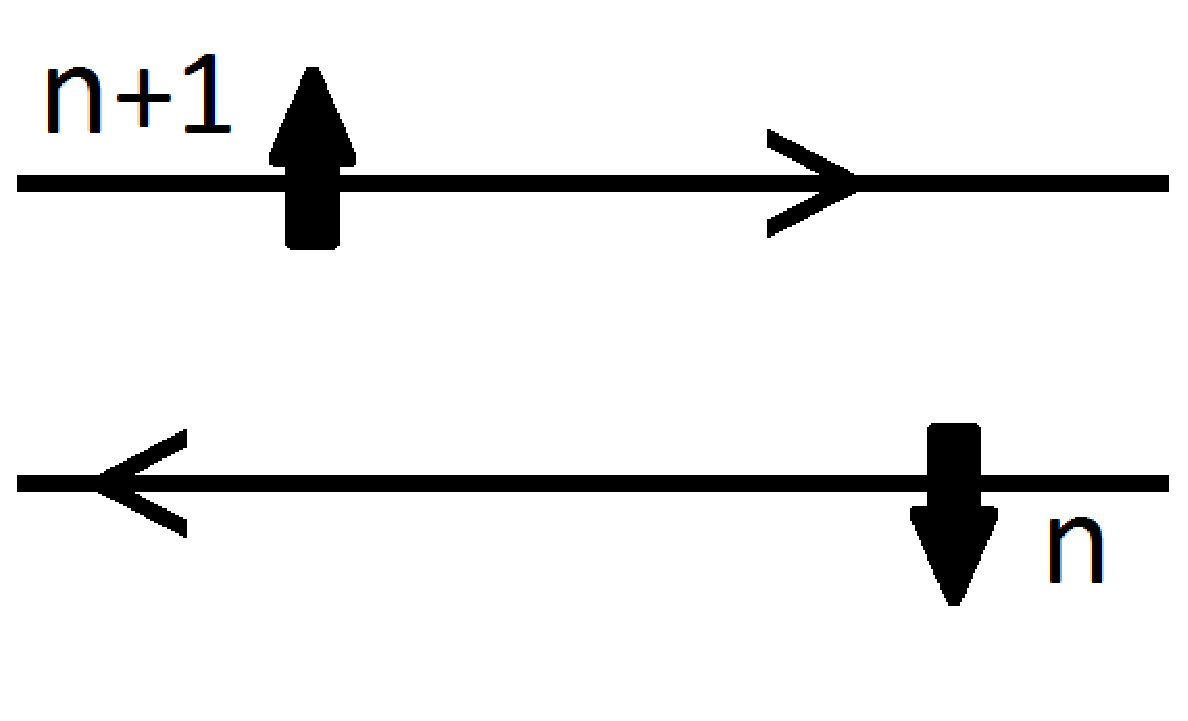
\includegraphics[width=1in]{apfig3}
\end{figure}

\[\Pi=\frac{k_F^{0,\downarrow}-k_F^{1,\uparrow}}{i\omega_n-(\omega_{\perp}-E_z)-\frac{1}{2\pi} \frac{V_0 q_\perp^2}{\omega_{\perp}} (k_F^{0,\downarrow}+k_F^{0,\uparrow}-3k_F^{1,\uparrow})}\]

\begin{figure}[h]
	\centering
	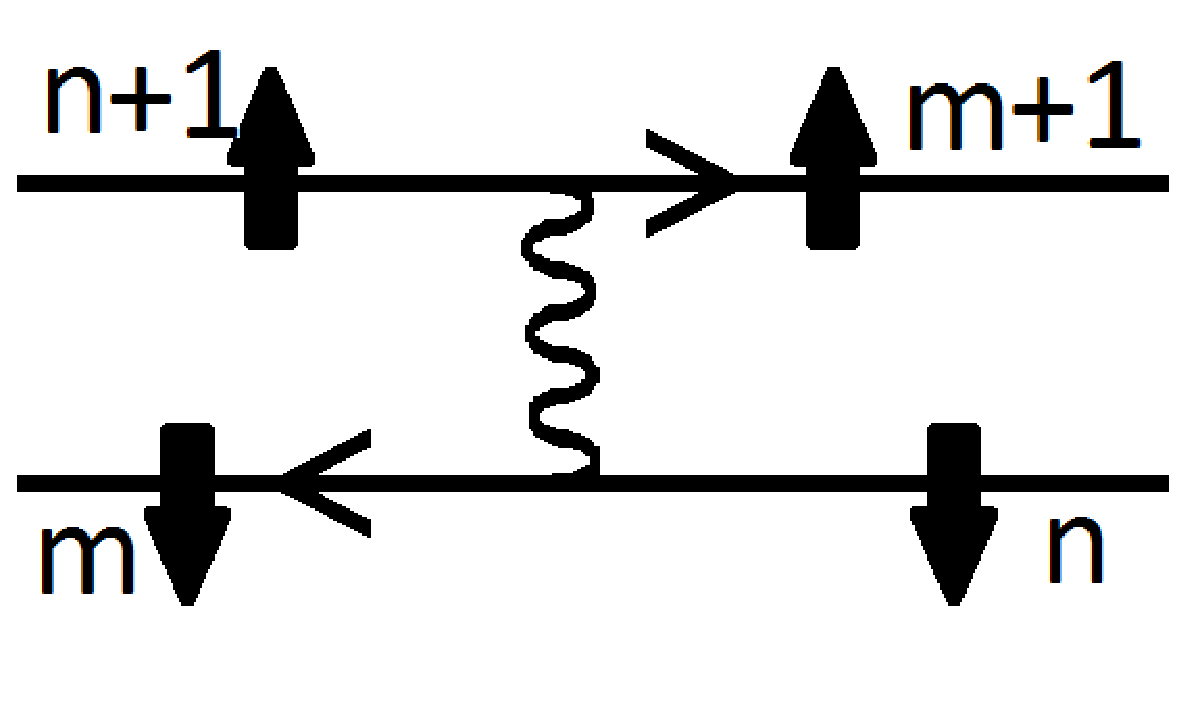
\includegraphics[width=1in]{apfig4}
\end{figure}

\[V=\frac{1}{2} V_0 q_\perp^2 \left( \langle 0|y^2|0\rangle + \langle 1|y^2|1\rangle \right) = \frac{1}{2} \frac{V_0 q_\perp^2}{\omega_{\perp}} (2)\]

\[V.\Pi|_{\omega\rightarrow (\omega_{\perp}-E_z)}=\frac{(k_F^{0,\downarrow}-k_F^{1,\uparrow}) . \frac{V_0 q_\perp^2}{\omega_{\perp}}}{-\frac{1}{2\pi} \frac{V_0 q_\perp^2}{\omega_{\perp}} (k_F^{o,\downarrow}+k_F^{0,\uparrow}-3k_F^{1,\uparrow})}\neq -1\]

\[det(\mathbb{I}+V\Pi)|_{\omega\rightarrow (\omega_{\perp}-E_z)}\neq0\]

\section{Local Interaction, $|n+1,\uparrow\rangle,|n,\downarrow\rangle$ Pair}

\[V\equiv V_0 \delta(y_1-y_2)\]

\[\Sigma_{n,\downarrow}=(V_\rho-3V_s)\sum\limits_{m=0}^N\frac{k_F^{m,\uparrow}}{\pi}\int\phi_n^2(y)\phi_m^2(y)dy\]

\[\Sigma_{n+1,\uparrow}=(V_\rho-3V_s)\sum\limits_{m=0}^{N+1}\frac{k_F^{m,\downarrow}}{\pi}\int\phi_{n+1}^2(y)\phi_m^2(y)dy\]

\[\Pi_n=\frac{\frac{1}{\pi}(k_F^{n,\downarrow}-k_F^{n+1,\uparrow})}{i\omega_n-(\omega_{\perp}-E_z)+\Sigma_{n,\downarrow}-\Sigma_{n+1,\uparrow}}\]

\[V=(V_\rho-3V_s)\int\phi_{n+1}\phi_{m+1}\phi_n\phi_m dy\]

%%%%%%%%%%%%%%%%%%%%%%%%%%%%%%%%%%%%%%%%%%%%%%%%%%%%%%%%%%%%%%%%%%%%%%%%%%
% Spin-Orbit%%%%%%%%%%%%%%%%%%%%%%%%%%%%%%%%%%%%%%%%%%%%%%%%%%%%%%%%%%%%%%
%%%%%%%%%%%%%%%%%%%%%%%%%%%%%%%%%%%%%%%%%%%%%%%%%%%%%%%%%%%%%%%%%%%%%%%%%%

\section{Local Interaction with SO coupling}

The Hamiltonian:

\begin{equation}
	H= \frac{p_x^2+p_y^2}{2m_e} +V_c(y)- \frac{1}{2} E_z \sigma_z + \alpha_- p_y \sigma_x
\end{equation}

The eigenstates and eigenvectors are:

\begin{equation}
	\begin{split}
		&|\psi_{n,+}\rangle = \alpha_n |\phi_{n+1}^+\rangle + \beta_n |\phi_n^-\rangle \\
	&|\psi_{n,-}\rangle = \beta_n^* |\phi_{n+1}^+\rangle - \alpha_n^* |\phi_n^-\rangle
	\end{split}
\end{equation}

where,
\[\alpha_n=i cos\left(\frac{\theta_n}{2}\right),\ \beta_n=-sin\left(\frac{\theta_n}{2}\right),\ \theta_n =cos^{-1}\left[\frac{E_z-\omega_{\perp}}{\sqrt{(E_z-\omega_{\perp})^2+\left[\delta_n^{SO}\right]^2}}\right] \]
%%%%%%%%%%%%%%%%%%%%%%%%%%%%%%%%%%%%%%%%%%%%%%%%%%%%%%%%%%%%%%%%%%%%%%%%%%%%%%%%%%%%%
%%%%%%%%%%%%%%%%%%%%%%%%%%%%%%%%%%%%%%%%%%%%%%%%%%%%%%%%%%%%%%%%%%%%%%%%%%%%%%%%%%%%%
%%%%%%%%%%%%%%%%%%%%%%%%%%%%%%%%%%%%%%%%%%%%%%%%%%%%%%%%%%%%%%%%%%%%%%%%%%%%%%%%%%%%%

\section{The Equation of the``Theory" Curve}

We have, 

\be F_0=\frac{1}{2} (V_\rho-3V_s) N(0) \equiv \frac{1}{2} \overline{V} \frac{m}{\pi} \ee

\be G_0=-\frac{1}{2} (V_\rho-3V_s) N(0) \equiv -\frac{1}{2} \overline{V} \frac{m}{\pi} \ee

Thus, $F_0=-G_0 \\$

Then we have,

\[ \omega_{th}=\pm \left[ {E_z + E_z \frac{G_1-G_0}{2(1+G_0)} - \sqrt{E_z^2 \frac{(G_1-G_0)^2}{4(1+G_0)^2}+\omega_{\perp}^2 \frac{G_1+1}{F_1+1} \frac{G_0+1}{F_0+1}}} \right] \]
\be \Rightarrow \omega_{th}= \pm \left[ {E_z + E_z \frac{\overline{V}\frac{m}{\pi}}{4\left(1-\frac{1}{2}\overline{V}\frac{m}{\pi}\right)}-\sqrt{E_z^2 \frac{\left( \overline{V} \frac{m}{\pi} \right)^2}{16\left(1-\frac{1}{2}\overline{V}\frac{m}{\pi}\right)^2}+\omega_{\perp}^2\left( \frac{1-\frac{1}{2}\overline{V}\frac{m}{\pi}}{1+\frac{1}{2}\overline{V}\frac{m}{\pi}}\right)} } \right]\ee

\section{Eigenvalue Scheme for Computation (for $|n+1,\uparrow\rangle , |n,\downarrow\rangle$ Pair)}

We are interested in the zeroes of the matrix $\left[ \Pi^{-1}+V \right]$, which is:

\begin{align*}
& \left[ \Pi^{-1}+V \right]_{nn'} \\ 
= &\frac{\omega-(\omega_{\perp}-E_z)+\frac{\overline{V}}{\pi} \sum\limits_m \left( \frac{k_F^{m,\uparrow}}{\pi}\int\phi_n^2(y)\phi_m^2(y)dy - \frac{k_F^{m,\downarrow}}{\pi}\int\phi_{n+1}^2(y)\phi_m^2(y)dy \right)}{\frac{1}{\pi} \left( k_F^{n,\downarrow}-k_F^{n+1,\uparrow} \right)} \delta_{nn'} \\
&+ \overline{V} \int\phi_{n+1}\phi_{n'+1}\phi_n\phi_{n'} dy \\
 = &\left( \omega-(\omega_{\perp}-E_z)+\frac{\overline{V}}{\pi} \sum\limits_m \left( \frac{k_F^{m,\uparrow}}{\pi}\int\phi_n^2(y)\phi_m^2(y)dy - \frac{k_F^{m,\downarrow}}{\pi}\int\phi_{n+1}^2(y)\phi_m^2(y)dy \right) \right)\delta_{nn'} \\
 &+ \frac{1}{\pi} \left( k_F^{n,\downarrow}-k_F^{n+1,\uparrow} \right) \overline{V} \int\phi_{n+1}\phi_{n'+1}\phi_n\phi_{n'} dy 
\end{align*}

We define, smatrix $\Rightarrow \frac{1}{\pi} \sum\limits_m \left( \frac{k_F^{m,\uparrow}}{\pi}\int\phi_n^2(y)\phi_m^2(y)dy - \frac{k_F^{m,\downarrow}}{\pi}\int\phi_{n+1}^2(y)\phi_m^2(y)dy \right)\delta_{nn'}$

kmatrix $\Rightarrow \frac{1}{\pi} \left(k_F^{n,\downarrow}-k_F^{n+1,\uparrow} \right).\delta_{nn'}$

vmatrix $\Rightarrow \int\phi_{n+1}\phi_{n'+1}\phi_n\phi_{n'} dy $

$M\equiv \mathrm{-smatrix-kmatrix.vmatrix} $

With these definitions, we can write for zeroes of $\left[ \Pi^{-1}+V\right]$ : 

\[ \mathrm{det} \left[ \frac{1}{\overline{V}} \left( \omega-(\omega_{\perp}-E_z) \right).\mathbbm{1}-M \right] =0  \]

As this is an eigenvalue equation with eigenvalues $\lambda = \frac{1}{\overline{V}} \left( \omega-(\omega_{\perp}-E_z) \right)$, it has solutions:

\be \omega_n = \overline{V}.\left[ \mathrm{Eigenvalues}[M] \right]_n + (\omega_{\perp}-E_z) \ee
%%%%%%%%%%%%%%%%%%%%%%%%%%%%%%%%%%%%%%%%%%
\section{The Kohn Modes}

\subsection{$|n,\uparrow\rangle, |n,\downarrow\rangle$ Pair}

\[\Sigma_{n,\uparrow}=-V_0 \sum\limits_{m=0}^N \{(\beta+\alpha) \frac{k_F^{m,\uparrow}}{\pi} \int\phi_n^2\phi_m^2 dy + 2\alpha \frac{k_F^{m,\downarrow}}{\pi} \int \phi_n^2 \phi_m^2 dy\}\]

\[\Sigma_{n,\downarrow}=-V_0 \sum\limits_{m=0}^N \{2\alpha \frac{k_F^{m,\uparrow}}{\pi} \int\phi_n^2\phi_m^2dy (\beta+\alpha) \frac{k_F^{m,\downarrow}}{\pi} \int\phi_n^2\phi_m^2dy\}\]

\[\Pi_n=\frac{\frac{1}{\pi}(k_F^{n,\downarrow}-k_F^{n,\uparrow})}{\omega-E_z + \Sigma_{n,\downarrow}-\Sigma_{n,\uparrow}}\]

\[V=V_0 (\beta-\alpha) \int\phi_n^2\phi_m^2dy\]

\subsection{$|n\rangle, |n+1\rangle$ Pair}

\[\Sigma_{n,\uparrow}=-\frac{V_0}{\pi} \sum\limits_{m=0}^N \{(\beta+\alpha) k_F^{m,\uparrow} + 2\alpha k_F^{m,\downarrow}\} \int\phi_n^2\phi_m^2dy\]

\[\Sigma_{n+1,\uparrow}=-\frac{V_0}{\pi} \sum\limits_{m=0}^N \{(\beta+\alpha) k_F^{m,\uparrow} + 2\alpha k_F^{m,\downarrow}\} \int\phi_{n+1}^2\phi_m^2dy\]


\[\Sigma_{n,\downarrow}=-\frac{V_0}{\pi} \sum\limits_{m=0}^N \{(\beta+\alpha) k_F^{m,\downarrow} + 2\alpha k_F^{m,\uparrow}\} \int\phi_n^2\phi_m^2dy\]

\[\Sigma_{n+1,\downarrow}=-\frac{V_0}{\pi} \sum\limits_{m=0}^N \{(\beta+\alpha) k_F^{m,\downarrow} + 2\alpha k_F^{m,\uparrow}\} \int\phi_{n+1}^2\phi_m^2dy\]

\[\Pi_{n,\uparrow}^{n+1,\uparrow}=\frac{\frac{1}{\pi}(k_F^{n,\uparrow}-k_F^{n+1,\uparrow})}{\omega-\omega_{\perp}+\Sigma_{n,\uparrow}-\Sigma_{n+1,\uparrow}}\]

\[\Pi_{n,\downarrow}^{n+1,\downarrow}=\frac{\frac{1}{\pi}(k_F^{n,\downarrow}-k_F^{n+1,\downarrow})}{\omega-\omega_{\perp}+\Sigma_{n,\downarrow}-\Sigma_{n+1,\downarrow}}\]

\[V_{nm} (\mathrm{1^{st}\ and\ 4^{th}\ block}): V_0 (\beta+\alpha) \int\phi_{n+1}\phi_{m+1}\phi_n\phi_mdy\]

\[V_{nm} (\mathrm{2^{nd}\ and\ 3^{rd}\ block}): V_0 (2\alpha) \int\phi_{n+1}\phi_{m+1}\phi_n\phi_mdy\]



